%!TEX TS-program = xelatex
%!TEX encoding = UTF-8 Unicode

\documentclass[tikz,border=1]{standalone}
\usetikzlibrary{calc,positioning}

\begin{document}
  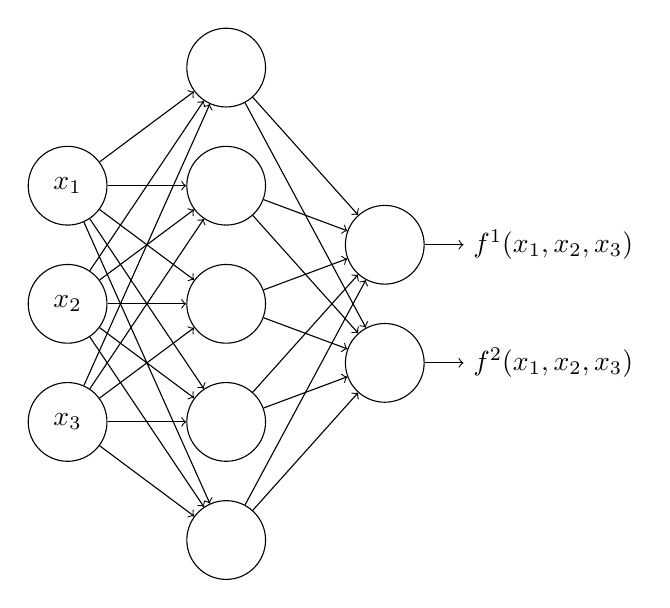
\begin{tikzpicture}[
    neuron/.style={circle,draw,inner sep=0pt,minimum size=10mm}
    ]
    
    \foreach \y in {0,...,4}
      \node (m\y) [neuron] at (0, \y * 1.5) {};

    \node (l0) [neuron,left=of m1] {$x_3$};
    \node (l1) [neuron,left=of m2] {$x_2$};
    \node (l2) [neuron,left=of m3] {$x_1$};
    
    \node (r0) [neuron,right=of m1,yshift=0.75cm] {};
    \node (r1) [neuron,right=of m3,yshift=-0.75cm] {};
    
    \foreach \x in {0,1,2}
      \foreach \y in {0,...,4}
        \draw[->] (l\x) to (m\y);

    \foreach \x in {0,...,4}
      \foreach \y in {0,1}
        \draw[->] (m\x) to (r\y);

    \draw[->] (r0) -- ++(1,0) node [right] {$f^2(x_1,x_2,x_3)$};
    \draw[->] (r1) -- ++(1,0) node [right] {$f^1(x_1,x_2,x_3)$};

  \end{tikzpicture} 
\end{document}
